\subsection{Parallelism of Pipeline Join}\label{sec:experiments_join}
We studied the scalability of SeqStar's pipeline join algorithm on two of the most time-consuming queries $q_6$ and $q_8$ (Figure).

\begin{figure}[ht]
  \centering
  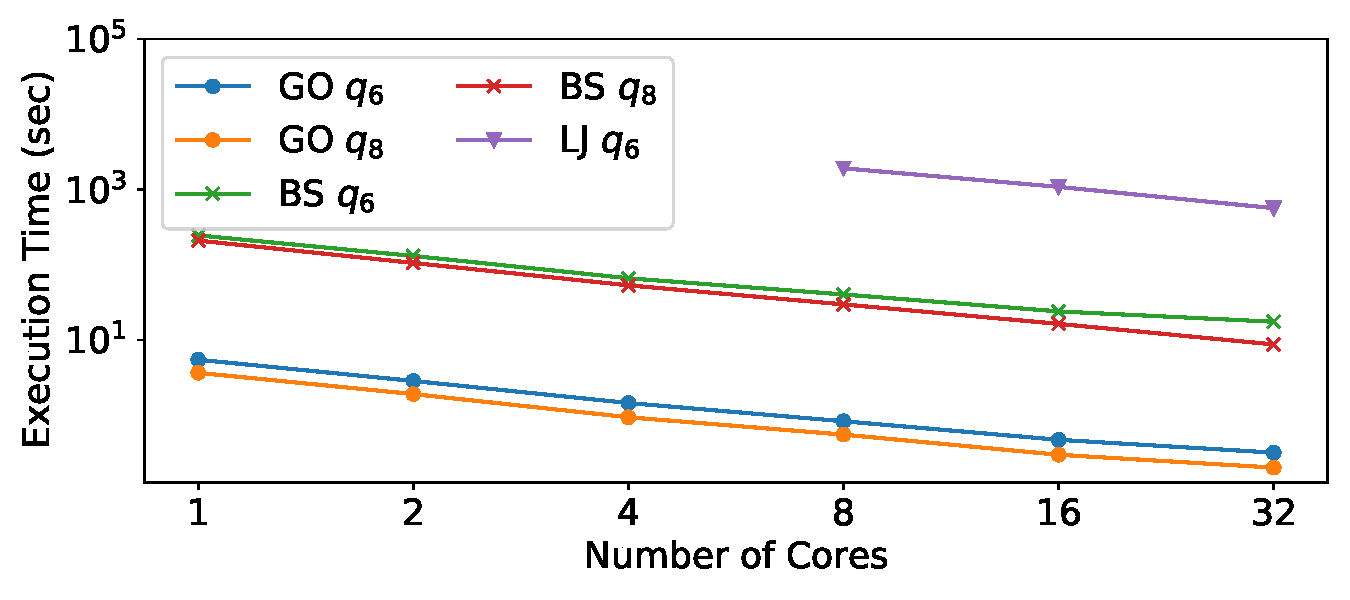
\includegraphics[width=0.5\textwidth]{img/exp_scalability.pdf}
  \caption{Scalability of Pipeline Join.}\label{img:exp_scalability}
\end{figure}

\subsection{Performance of Predicate Pushdown}
In order to understand the benefits of predicate pushdown,
we ran the four of the most time-consuming queries $q_4$, $q_5$, $q_6$ and $q_8$ with a WHERE clause:
\begin{Verbatim}[fontsize=\small]
  WHERE u1 % 5 = 0 AND u2 % u1 = 5
\end{Verbatim}
The analyzer of SeqStar will analyze the WHERE clause and extract the filtering constraints:
$u_1 \bmod 5 = 0$ and $u_2 \bmod u_1 = 5$.
These filters can be applied during the star matching process.

\begin{table}
  \caption{Performance of Predicate Pushdown (LJ)}\label{tab:pushdown_lj}
  \begin{tabular}{lrrrrrr}
    \toprule
    $q$ & \parbox{5mm}{$T$ (sec)} & \parbox{5mm}{$T_{OPT}$ (sec)} & $\frac{T}{T_{OPT}}$ & $\#R$ & $\#R_{OPT}$ & $\frac{\#R}{\#R_{OPT}}$ \\
    \midrule
    4 &   944 &        11 &       89 &   1.0 $\times$ 10^{12} &   6.6 $\times$ 10^7 &     15376 \\
    5 & >2100 &         4 &     >525 &  3.2 $\times$ 10^{13}  &   6.7 $\times$ 10^8 &     47520 \\
    6 &   571 &        24 &       24 &   6.2 $\times$ 10^{11} &   1.6 $\times$ 10^8 &      3774 \\
    8 &  1513 &        24 &       63 &   1.7 $\times$ 10^{13} &    2.0 $\times$ 10^9&      8512 \\
    \bottomrule
  \end{tabular}
\end{table}

\begin{table}
  \caption{Performance of Predicate Pushdown (OK)}\label{tab:pushdown_ok}
  \begin{tabular}{lrrrrrr}
    \toprule
    $q$ & \parbox{5mm}{$T$ (sec)} & \parbox{5mm}{$T_{OPT}$ (sec)} & $\frac{T}{T_{OPT}}$ & $\#R$ & $\#R_{OPT}$ & $\frac{\#R}{\#R_{OPT}}$ \\
    \midrule
    4 & >2100 &        65 &      >32 &  5.6 $\times$ 10^{13} &   1.7 $\times$ 10^{10} &      3110 \\
    5 & >2100 &         7 &     >300 &  3.8 $\times$ 10^{14} &     4.6 $\times$ 10^8 &     813540 \\
    6 &  1399 &        38 &       37 &  4.4 $\times$ 10^{10} &     8.3 $\times$ 10^5 &      53035 \\
    8 &  1347 &        36 &       38 &  1.4 $\times$ 10^{13} &     6.1 $\times$ 10^8 &      22609 \\
    \bottomrule
  \end{tabular}
\end{table}
